% \textbf{\underline{OZ 7 - Inductantie - Oefening 4:}}
% \vspace{0.5cm}

% De schakelaar in Figuur 7.2 wordt gesloten op tijdstip $ t = 0 $ s. Bepaal de stroom door de spoel en de stroom door de schakelaar $ S $ in functie van $ t > 0 $.

% \begin{figure}[H]
%     \centering
%     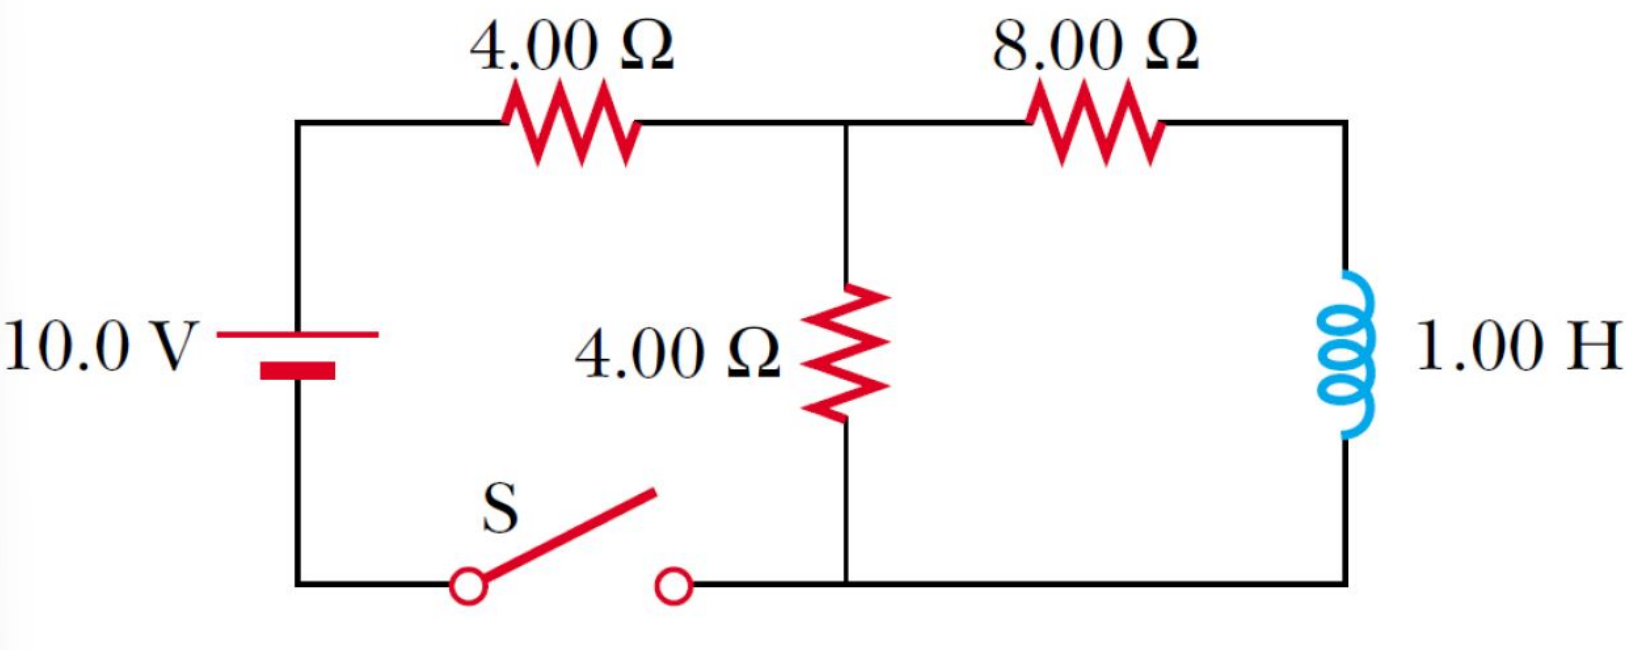
\includegraphics[width=8cm]{oz07/resources/oef-4-opgave.png}
    
%     \textbf{Figuur 7.2}
% \end{figure}

% \begin{description}[labelwidth=1.5cm, leftmargin=!]
%     \item[Geg. :]   $ \varepsilon = 10,0 $ V; $ R_1 = 4,00 \ \Omega$; $ R_2 = 4,00 \ \Omega $; $ R_3 = 8,00 \ \Omega $; $ L = 1,00 $ H;
% \end{description}

% \begin{figure}[H]
%     \centering
%     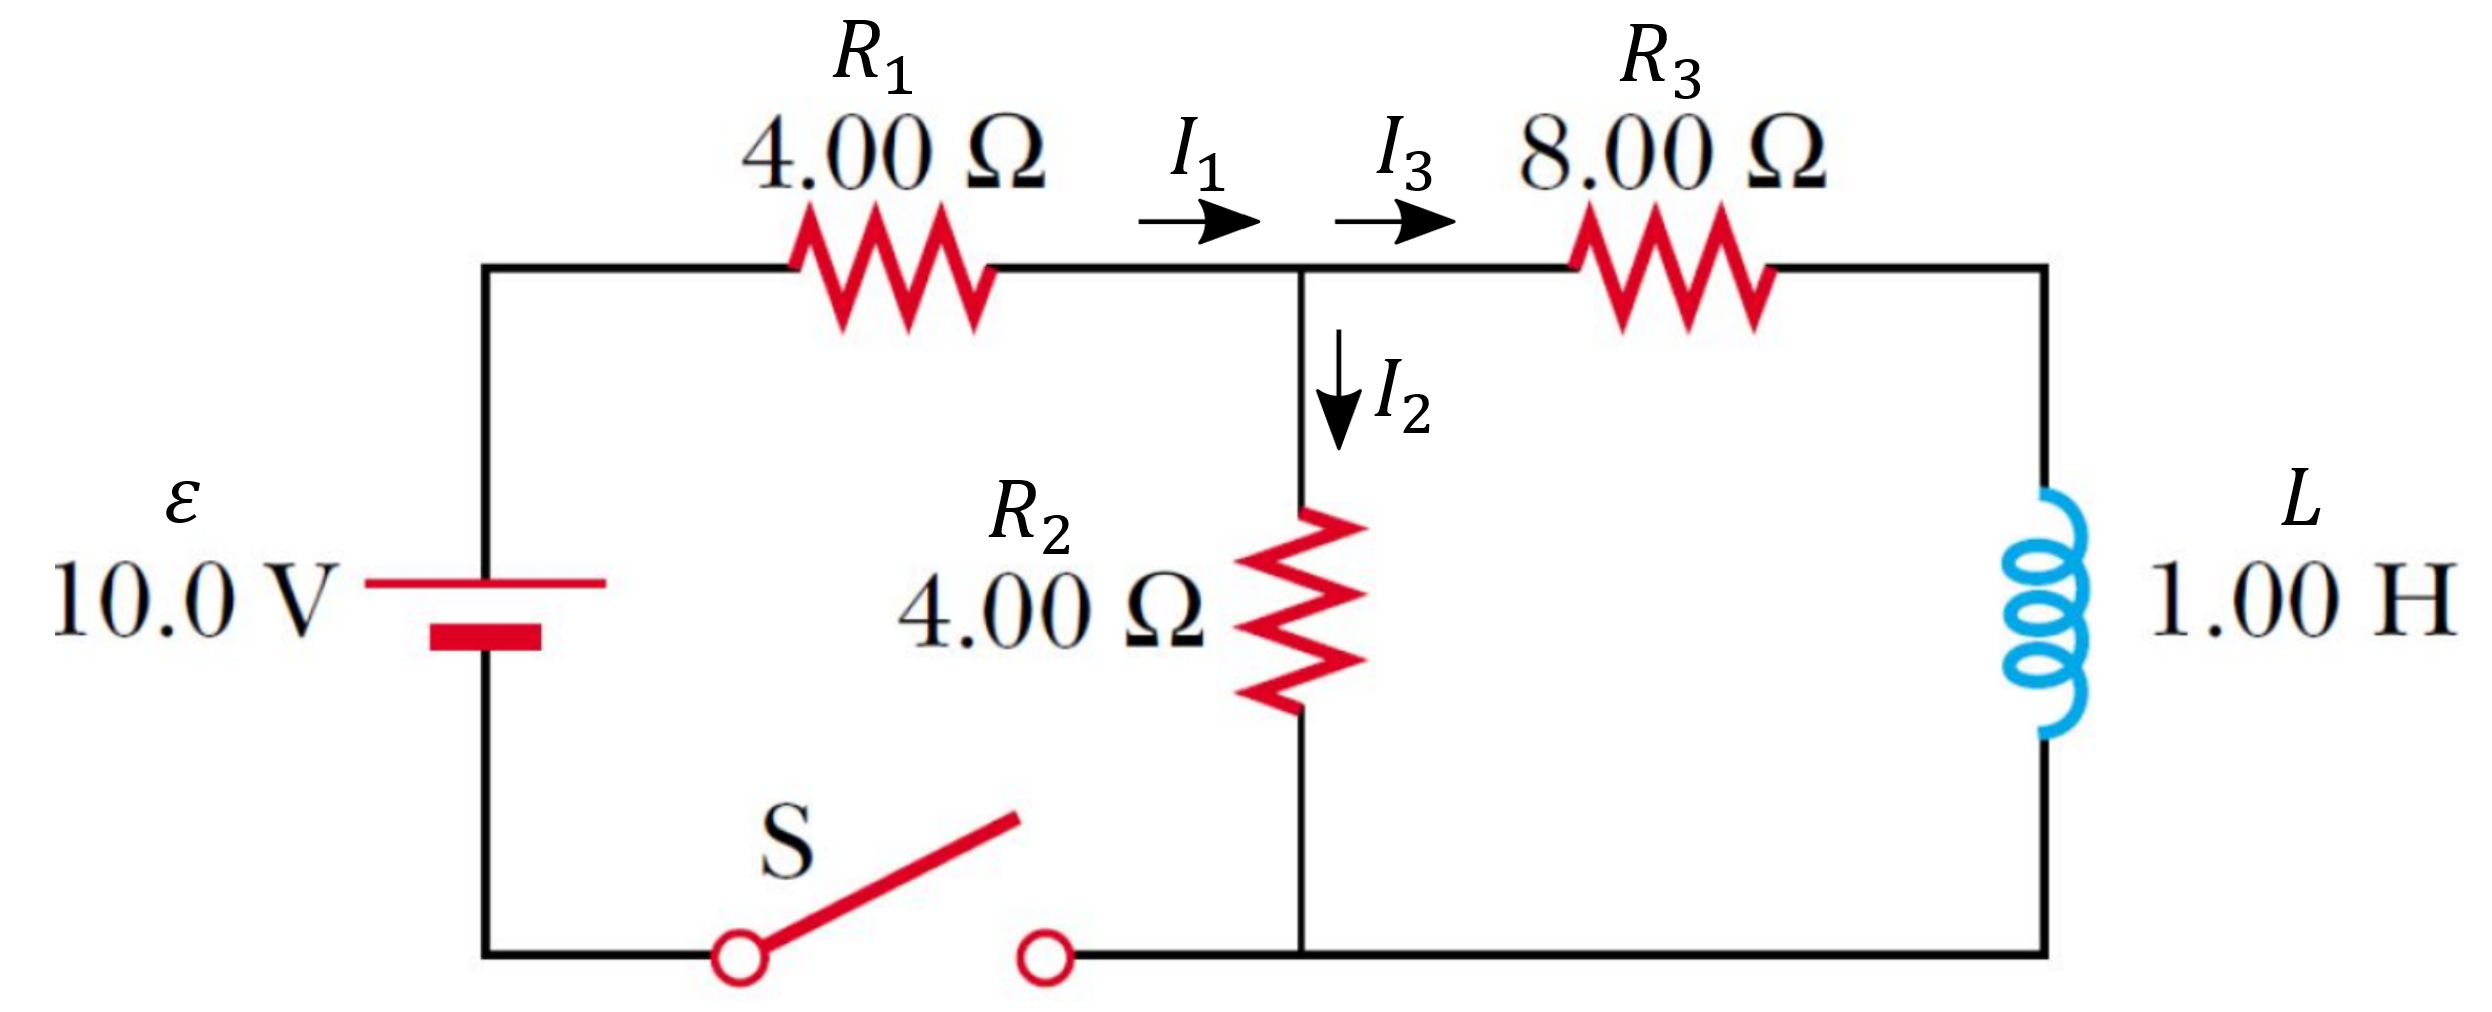
\includegraphics[width=8.3cm]{oz07/resources/oef-4-schets.png}
    
%     \textbf{Schets 7.1}
% \end{figure}

% \begin{description}[labelwidth=1.5cm, leftmargin=!]
%     \item[Gevr. :]  $ I_1 $; $ I_3 $;
%     \item[Opl. :]   $ \left\{\begin{array}{l}
%                         \varepsilon = I_1 R_1 + I_2 R_2 \\
%                         I_2 R_2 = I_3 R_3 + L \dfrac{dI_3}{dt} \\
%                         I_1 = I_2 + I_3
%                     \end{array}\right. $
                    
%                     \hspace{-0.57cm} $ \Rightarrow
%                     \left\{\begin{array}{l}
%                         \varepsilon = \left( I_2 + I_3 \right) R_1 + I_2 R_2 \\
%                         I_2 R_2 = I_3 R_3 + L \dfrac{dI_3}{dt} \\
%                         I_1 = I_2 + I_3
%                     \end{array}\right. $
                    
%                     \hspace{-0.57cm} $ \Rightarrow
%                     \left\{\begin{array}{l}
%                         \varepsilon = I_2 \left( R_1 + R_2 \right) + I_3 R_1 \\
%                         I_2 R_2 = I_3 R_3 + L \dfrac{dI_3}{dt} \\
%                         I_1 = I_2 + I_3
%                     \end{array}\right. $
                    
%                     \hspace{-0.57cm} $ \Rightarrow
%                     \left\{\begin{array}{l}
%                         I_2 = \dfrac{\varepsilon - I_3 R_1}{R_1 + R_2} \\
%                         I_2 R_2 = I_3 R_3 + L \dfrac{dI_3}{dt} \\
%                         I_1 = I_2 + I_3
%                     \end{array}\right. $
                    
%                     \hspace{-0.57cm} $ \Rightarrow 
%                     \dfrac{\varepsilon - I_3 R_1}{R_1 + R_2} R_2 = I_3 R_3 + L \dfrac{dI_3}{dt} $
                    
%                     \hspace{-0.57cm} $ \Leftrightarrow 
%                     \dfrac{\varepsilon}{R_1 + R_2} R_2 - \dfrac{I_3 R_1}{R_1 + R_2} R_2 = I_3 R_3 + L \dfrac{dI_3}{dt} $
                    
%                     \hspace{-0.57cm} $ \Leftrightarrow 
%                     \dfrac{\varepsilon}{R_1 + R_2} R_2 - \dfrac{R_1 R_2}{R_1 + R_2} I_3 = I_3 R_3 + L \dfrac{dI_3}{dt} $
                    
%                     \hspace{-0.57cm} $ \Leftrightarrow 
%                     L \dfrac{dI_3}{dt} + \left( R_3 + \dfrac{R_1 R_2}{R_1 + R_2} \right) I_3 - \dfrac{\varepsilon}{R_1 + R_2} R_2 = 0 $
                    
%                     \hspace{-0.57cm} $ \Leftrightarrow 
%                     \dfrac{dI_3}{dt} + \left( R_3 + \dfrac{R_1 R_2}{R_1 + R_2} \right) \dfrac{I_3}{L} - \dfrac{R_2}{R_1 + R_2} \dfrac{\varepsilon}{L} = 0 $
                    
%                     \hspace{-0.57cm} $ \Leftrightarrow 
%                     \dfrac{dI_3}{dt} + \left( 8,00 + \dfrac{4,00 \cdot 4,00}{4,00 + 4,00} \right) \dfrac{I_3}{1,00} - \dfrac{4,00}{4,00 + 4,00} \dfrac{10,0}{1,00} = 0 $
                    
%                     \hspace{-0.57cm} $ \Leftrightarrow 
%                     \dfrac{dI_3}{dt} + 10 I_3 - 5 = 0 $
                    
%                     \hspace{-0.57cm} $ \Rightarrow 
%                     I_3{\left( t \right)} = c \cdot e^{-10t} - \dfrac{-5}{10} = c \cdot e^{-10t} + 0,5 $
                    
%                     \vspace{0.5cm}
                    
%                     $ I_3{\left(t = 0 \textrm{ s} \right)} = 0 $ A
                    
%                     \hspace{-0.57cm} $ \Leftrightarrow 
%                     c \cdot e^{-10 \cdot 0} + 0,5 = 0 $
                    
%                     \hspace{-0.57cm} $ \Leftrightarrow 
%                     c = -0,5 $
                    
%                     \hspace{-0.57cm} $ \Rightarrow 
%                     I_3{\left( t \right)} = -0,5 \cdot e^{-10t} + 0,5 $
                    
%                     \vspace{0.5cm}
                    
%                     $ I_2 = \dfrac{\varepsilon - I_3 R_1}{R_1 + R_2} = \dfrac{10 - \left( -0,5 \cdot e^{-10t} + 0,5 \right) \cdot 4,00}{4,00 + 4,00} = \dfrac{10 + 2 \cdot e^{-10t} - 2 }{4,00 + 4,00} = 1 + 0,25 \cdot e^{-10t} $
                    
%                     \vspace{0.5cm}
                    
%                     $ I_1 = I_2 + I_3 = 1 + 0,25 \cdot e^{-10t} + -0,5 \cdot e^{-10t} + 0,5 = 1,50 - 0,250 \cdot e^{-10,0t} $
% \end{description}

% \vspace{1cm}